\documentclass{article}
\usepackage{iftex}
\ifluatex
	\usepackage{fontspec}
\else
	\usepackage[utf8]{inputenc} %Eingabekodierung nach UTF8-Unicode, Erlaubt direkte Eingabe von Umlauten etc.
\fi
\usepackage{amssymb}
\usepackage{amsmath}
\usepackage[ngerman]{babel}
\usepackage{csquotes}

\usepackage[headheight=24pt,heightrounded]{geometry}
\usepackage{graphicx}
\usepackage{titlesec}
\usepackage{fancyhdr}
\usepackage{enumerate}
\usepackage{listings}

\lstdefinestyle{mystyle}{
	keywordstyle=\color{magenta},
	basicstyle=\ttfamily\footnotesize,
	breakatwhitespace=false,         
	breaklines=true,                 
	captionpos=b,                    
	keepspaces=true,                 
	numbers=left,                    
	numbersep=5pt,                  
	showspaces=false,                
	showstringspaces=false,
	showtabs=false,                  
	tabsize=2
}
\lstset{style=mystyle}


\usepackage{xcolor}
\definecolor{urlcolor}{RGB}{0,136,204}
\definecolor{linkcolor}{RGB}{204,0,34}
\usepackage[colorlinks,urlcolor=urlcolor,linkcolor=linkcolor]{hyperref}

% TODOs
\usepackage[colorinlistoftodos,prependcaption,textsize=tiny]{todonotes}

% coloneqq
\usepackage{mathtools}

\usepackage{qtree}

% Blank lines instead of indented first line
\setlength{\parindent}{0pt}
\setlength{\parskip}{\baselineskip}

\newcommand{\sheet}[1]{
\pagestyle{fancy}
\fancyhead[L]{Big Data Engineering  \\ Assignment 9}
\fancyhead[R]{Leo Forster \\ Maximilian Prinz \\ Bastian Simon}

\titleformat{\section}
{\normalfont\Large\bfseries}{\thesection.}{1em}{}

}

% Hier kommen Vorlesungs- und Dokumentspezifische Makros

\newcommand{\NN}{\mathbb{N}}
\newcommand{\ZZ}{\mathbb{Z}}
\newcommand{\QQ}{\mathbb{Q}}
\newcommand{\RR}{\mathbb{R}}
\newcommand{\CC}{\mathbb{C}}
\newcommand{\inv}{^{-1}}
\newcommand{\lpar}{\left(}
\newcommand{\rpar}{\right)}

\newcommand{\limn}{{\lim_{n\to\infty}}}
\sheet{1}
\begin{document}

\section{ER modelling}

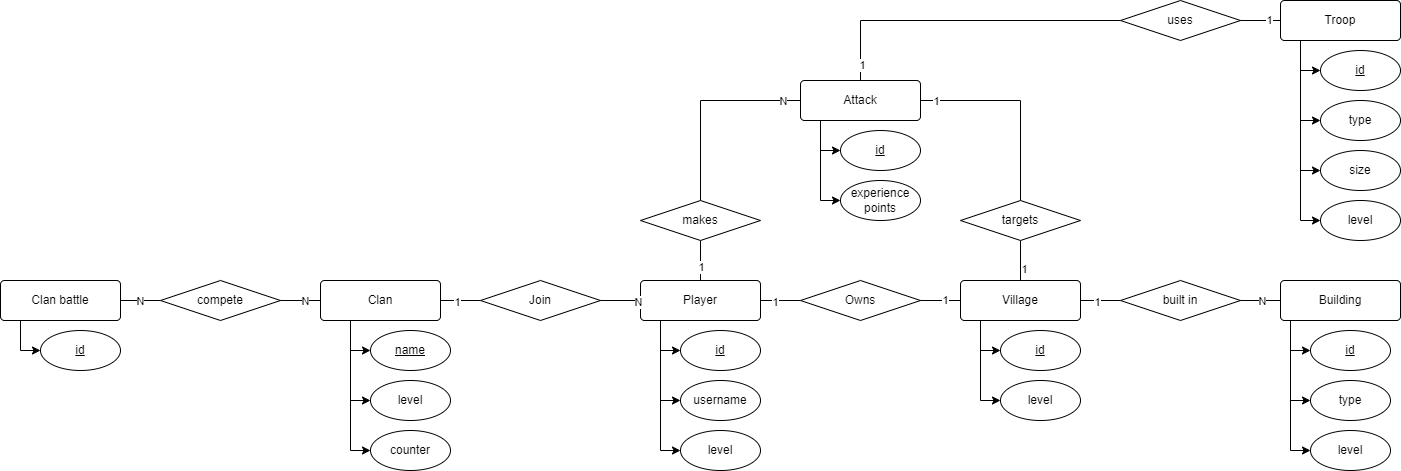
\includegraphics[width=\textwidth]{1.drawio.png}

\section{Design errors in ER modelling}

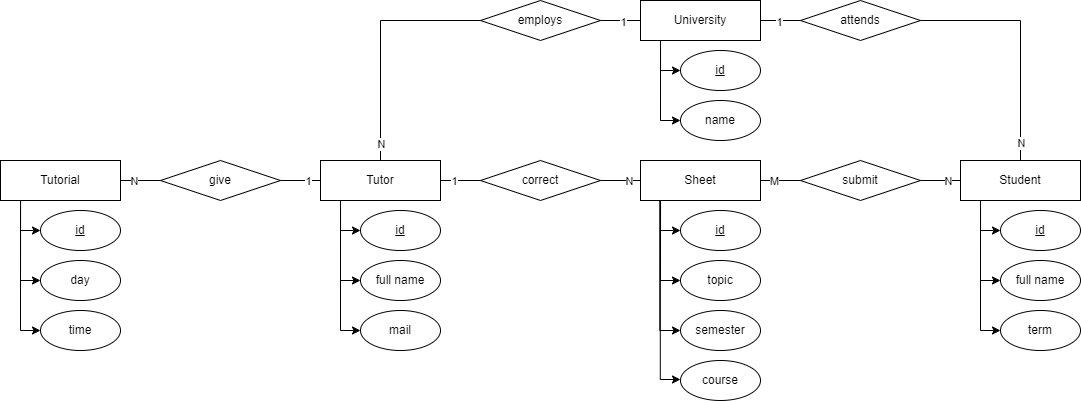
\includegraphics[width=\textwidth]{2.drawio.png}

\section{Ternary relationship}

\begin{itemize}
	\item[1.] False, because professors are denoted with 1, which means that in every term at most one professor can teach a course.
	\item[2.] False, because one course can at most be held by one professor in a single term.
	\item[3.] Correct. A professor can at most teach one course per term, because it is a 1:N relation.
	\item[4.] False. A professor could teach a course in one term and another one in another term. It is only said that a professor can at most teach one course in one term, not how many different courses he can teach in different terms.
	\item[5.] False. It is only said that a course can be held by at most one professor in one term. So professor A could teach course B in term 1 and 2. 
\end{itemize}

\section{IMDb singers}

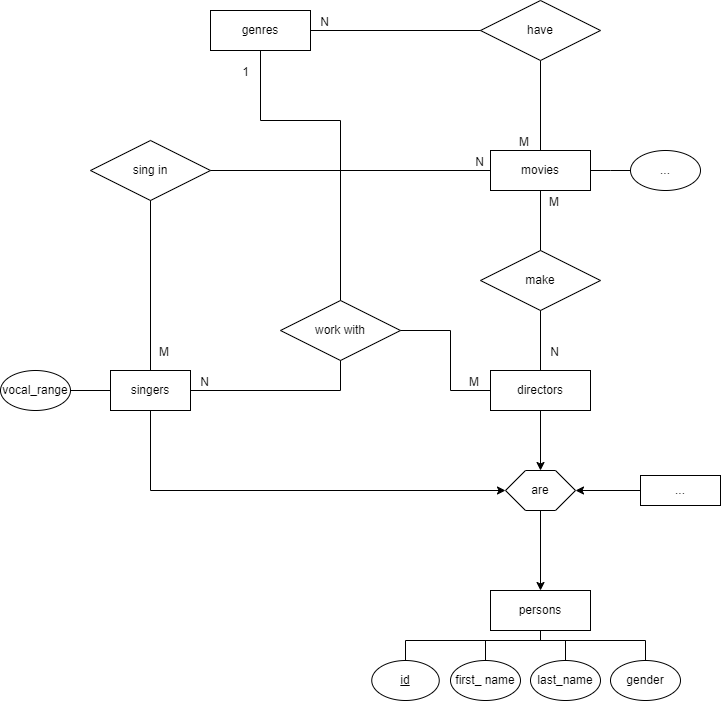
\includegraphics[width=\textwidth]{4.drawio.png}

\end{document}